\subsubsection{20.12.14}
\begin{enumerate}
	
	\item Время начала и окончания собрания: 17:00 - 20:00.
	
	\item Цели собрания: 
	\begin{enumerate}
		
		\item Скрепить новый ковш степлером.
		
		\item Установить укрепляющие пластины на нижнюю рейку подъемника.
		
		\item Демонтировать болт, способствующий разгону лопаток захвата мячей.
		
	\end{enumerate}
	\item Проделанная работа:
	\begin{enumerate}
		
		\item Новый ковш скреплен степлером и протестирован на предмет того, насколько легко шарики способны выкатываться из него. Результаты положительные: шарики выкатываются без проблем даже если в ковше больше пяти шариков.
		
		\begin{figure}[H]
			\begin{minipage}[h]{0.2\linewidth}
				\center  
			\end{minipage}
			\hfill
			\begin{minipage}[h]{0.29\linewidth}
				\center{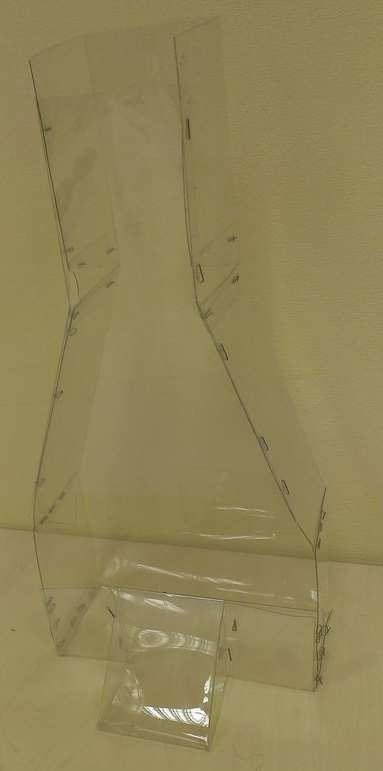
\includegraphics[scale=0.25]{days/20.12.14/images/01}}
			\end{minipage}
			\hfill
			\begin{minipage}[h]{0.29\linewidth}
				\center{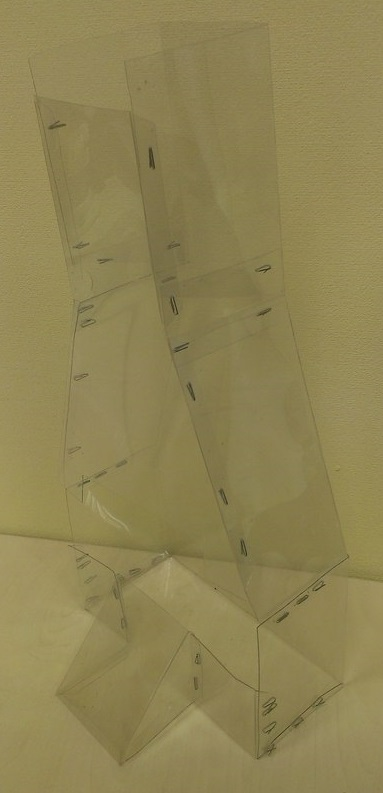
\includegraphics[scale=0.25]{days/20.12.14/images/02}}
			\end{minipage}
			\hfill
			\begin{minipage}[h]{0.2\linewidth}
				\center  
			\end{minipage}
			\caption{Новый ковш}
		\end{figure}
		
		\item Были отпилены укрепляющие пластины нужных размеров.
		
		\item Болт был демонтирован.
		
	\end{enumerate}
	
	\item Итоги собрания:
	\begin{enumerate}
		\item Ковш готов.
		
		\item Укрепляющие пластины готовы, но не закреплены.
		
		\item Болт демонтирован.
		
	\end{enumerate}
	
	\item Задачи для последующих собраний:
	\begin{enumerate}
		\item Закрепить укрепляющие пластины на нижнюю рейку подъемника.
		
		\item Заменить сломаный привод.
		
		\item Запаять концы проводов, соединяющих аккумулятор и приводы с драйверами.		
	\end{enumerate}
\end{enumerate}
\fillpage
